\chapter{Natural Deduction for Predicate Logic}\label{ch:preddeduction}

Natural deduction for predicate logic keeps all the propositional rules (now applied to
first-order formulas) and adds introduction and elimination rules for $\forall$, $\exists$
and $=$.

\section{Rules for the quantifiers}

\subsection{\texorpdfstring{$\forall$}{for all} elimination}
\[
  \dfrac{\forall x\,\varphi}{\varphi[t/x]}\ \forall e
  \qquad\text{($t$ any term free for $x$ in $\varphi$).}
\]
If something holds for everything, it holds for any particular $t$.

\subsection{\texorpdfstring{$\forall$}{for all} introduction}
\[
  \dfrac{\begin{array}{|c|}\hline x_0\ \text{(fresh)}\\ \vdots\\ \varphi[x_0/x]\\\hline\end{array}}
  {\forall x\,\varphi}\ \forall i
\]
Open a box with a \emph{fresh} variable $x_0$ that appears nowhere outside the box (not in
premises, not in open assumptions, not in the conclusion). If we can prove
$\varphi[x_0/x]$ about this completely arbitrary $x_0$, the proof works for every value,
so $\forall x\,\varphi$ follows. This is the formal version of ``let $x_0$ be arbitrary''.

\subsection{\texorpdfstring{$\exists$}{exists} introduction}
\[
  \dfrac{\varphi[t/x]}{\exists x\,\varphi}\ \exists i
  \qquad\text{($t$ free for $x$ in $\varphi$).}
\]
A concrete witness $t$ gives existence.

\subsection{\texorpdfstring{$\exists$}{exists} elimination}
\[
  \dfrac{\exists x\,\varphi\qquad
  \begin{array}{|c|}\hline x_0\quad \varphi[x_0/x]\ \text{(assumption)}\\ \vdots\\ \chi\\\hline\end{array}}
  {\chi}\ \exists e
\]
Knowing that \emph{some} object satisfies $\varphi$, give it a fresh name $x_0$, assume
$\varphi[x_0/x]$, and derive $\chi$. Provided $x_0$ does not occur in $\chi$ (or anywhere
outside the box), $\chi$ follows. This is like $\lor e$ over all possible witnesses.

\begin{important}[Freshness conditions]
\begin{itemize}
  \item In $\forall i$ and $\exists e$, the variable $x_0$ must be new: it must not occur
        in any premise, any open assumption, or the formula concluded after the box.
  \item In $\exists e$ the conclusion $\chi$ must not mention $x_0$: we do not know
        \emph{which} object the witness is.
  \item In $\forall e$ and $\exists i$, $t$ must be free for $x$ (no variable capture).
\end{itemize}
Violating these is the most common source of ``proofs'' of false statements, e.g.\
deriving $\forall x\,P(x)$ from $\exists x\,P(x)$ by using the witness as if it were
arbitrary.
\end{important}
Indeed $\exists x\,P(x)\not\models\forall x\,P(x)$, so by soundness no correct proof can
exist; a two-element interpretation shows it:
\begin{center}
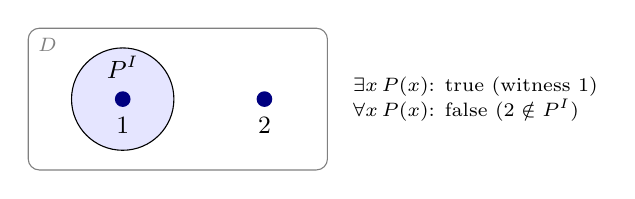
\begin{tikzpicture}[p/.style={circle,fill=blue!50!black,inner sep=2pt}]
  \draw[rounded corners,gray] (-1.2,-0.9) rectangle (2.6,0.9);
  \node[font=\scriptsize,gray,anchor=north west] at (-1.2,0.9) {$D$};
  \draw[fill=blue!10] (0,0) circle (0.65cm);
  \node[p,label=below:{\small $1$}] at (0,0) {};
  \node[p,label=below:{\small $2$}] at (1.8,0) {};
  \node[font=\small] at (0,0.4) {$P^I$};
  \node[font=\scriptsize,anchor=west,align=left] at (2.8,0) {$\exists x\,P(x)$: true (witness $1$)\\ $\forall x\,P(x)$: false ($2\notin P^I$)};
\end{tikzpicture}
\end{center}

\section{Rules for equality}
\[
  \dfrac{}{t=t}\ {=}i
  \qquad\qquad
  \dfrac{t_1=t_2\qquad\varphi[t_1/x]}{\varphi[t_2/x]}\ {=}e
\]
($t_1,t_2$ free for $x$ in $\varphi$.) $=e$ is ``substitution of equals for equals''.

\begin{example}[Symmetry of $=$: $t_1=t_2\vdash t_2=t_1$]
\begin{ndproof}
1 & $t_1=t_2$ & premise\\
2 & $t_1=t_1$ & $=i$\\
3 & $t_2=t_1$ & $=e$ 1, 2 \quad (with $\varphi$ being $x=t_1$)
\end{ndproof}
Transitivity ($t_1=t_2,\ t_2=t_3\vdash t_1=t_3$) is a single $=e$ with $\varphi$ being
$t_1=x$.
\end{example}

\section{Example proofs}

\begin{example}[$\forall x\,(P(x)\to Q(x)),\ \forall x\,P(x)\vdash\forall x\,Q(x)$]
\begin{ndproof}
1 & $\forall x\,(P(x)\to Q(x))$ & premise\\
2 & $\forall x\,P(x)$ & premise\\
3 & \bx $P(x_0)\to Q(x_0)$ & $x_0$ fresh;\ $\forall e$ 1\\
4 & \bx $P(x_0)$ & $\forall e$ 2\\
5 & \bx $Q(x_0)$ & $\to e$ 4, 3\\
6 & $\forall x\,Q(x)$ & $\forall i$ 3--5
\end{ndproof}
\end{example}

\begin{example}[$\forall x\,(P(x)\to Q(x)),\ \exists x\,P(x)\vdash\exists x\,Q(x)$]
\begin{ndproof}
1 & $\forall x\,(P(x)\to Q(x))$ & premise\\
2 & $\exists x\,P(x)$ & premise\\
3 & \bx $P(x_0)$ & assumption, $x_0$ fresh\\
4 & \bx $P(x_0)\to Q(x_0)$ & $\forall e$ 1\\
5 & \bx $Q(x_0)$ & $\to e$ 3, 4\\
6 & \bx $\exists x\,Q(x)$ & $\exists i$ 5\\
7 & $\exists x\,Q(x)$ & $\exists e$ 2, 3--6
\end{ndproof}
Note line 6: we must reach a formula without $x_0$ \emph{inside} the box before closing it.
\end{example}

\begin{example}[$\neg\exists x\,P(x)\vdash\forall x\,\neg P(x)$]
\begin{ndproof}
1 & $\neg\exists x\,P(x)$ & premise\\
2 & \bx\bx $P(x_0)$ & $x_0$ fresh;\ assumption\\
3 & \bx\bx $\exists x\,P(x)$ & $\exists i$ 2\\
4 & \bx\bx $\bot$ & $\neg e$ 3, 1\\
5 & \bx $\neg P(x_0)$ & $\neg i$ 2--4\\
6 & $\forall x\,\neg P(x)$ & $\forall i$ 2--5
\end{ndproof}
The outer box (lines 2--5) is the $\forall i$ box for $x_0$; the inner one (2--4) is the
$\neg i$ box.
\end{example}

\begin{example}[$\neg\forall x\,P(x)\vdash\exists x\,\neg P(x)$]
This direction needs classical reasoning (PBC).
\begin{ndproof}
1 & $\neg\forall x\,P(x)$ & premise\\
2 & \bx $\neg\exists x\,\neg P(x)$ & assumption\\
3 & \bx\bx\bx $\neg P(x_0)$ & $x_0$ fresh;\ assumption\\
4 & \bx\bx\bx $\exists x\,\neg P(x)$ & $\exists i$ 3\\
5 & \bx\bx\bx $\bot$ & $\neg e$ 4, 2\\
6 & \bx\bx $P(x_0)$ & PBC 3--5\\
7 & \bx $\forall x\,P(x)$ & $\forall i$ 3--6\\
8 & \bx $\bot$ & $\neg e$ 7, 1\\
9 & $\exists x\,\neg P(x)$ & PBC 2--8
\end{ndproof}
\end{example}

\begin{example}[$\exists x\,\forall y\,R(x,y)\vdash\forall y\,\exists x\,R(x,y)$]
\begin{ndproof}
1 & $\exists x\,\forall y\,R(x,y)$ & premise\\
2 & \bx $\forall y\,R(x_0,y)$ & assumption, $x_0$ fresh\\
3 & \bx\bx $R(x_0,y_0)$ & $y_0$ fresh;\ $\forall e$ 2\\
4 & \bx\bx $\exists x\,R(x,y_0)$ & $\exists i$ 3\\
5 & \bx $\forall y\,\exists x\,R(x,y)$ & $\forall i$ 3--4\\
6 & $\forall y\,\exists x\,R(x,y)$ & $\exists e$ 1, 2--5
\end{ndproof}
Trying to prove the converse fails exactly at a freshness condition: from
$\forall y\,\exists x\,R(x,y)$ we would get a witness $x_0$ depending on $y_0$, and could
not then generalise over $y_0$ while concluding something about $x_0$.
\end{example}

The boxes of the last proof, drawn with the fresh variable each one introduces in its corner:
\begin{center}
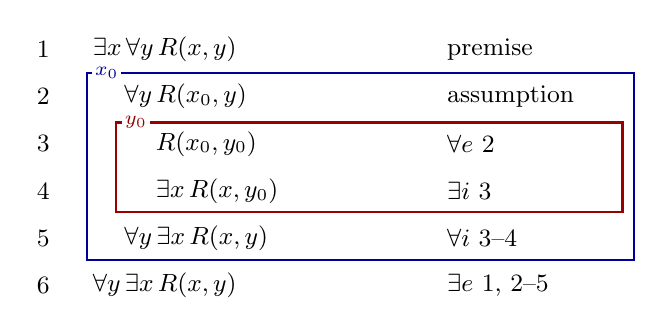
\begin{tikzpicture}[font=\small]
  \foreach \n/\f/\j/\ind in {1/{$\exists x\,\forall y\,R(x,y)$}/premise/0,2/{$\forall y\,R(x_0,y)$}/assumption/1,
      3/{$R(x_0,y_0)$}/{$\forall e$ 2}/2,4/{$\exists x\,R(x,y_0)$}/{$\exists i$ 3}/2,
      5/{$\forall y\,\exists x\,R(x,y)$}/{$\forall i$ 3--4}/1,6/{$\forall y\,\exists x\,R(x,y)$}/{$\exists e$ 1, 2--5}/0} {
    \node[anchor=east] at (0,-0.6*\n) {\n};
    \node[anchor=west] at (0.3+0.4*\ind,-0.6*\n) {\f};
    \node[anchor=west] at (4.8,-0.6*\n) {\j};
  }
  \draw[thick,blue!60!black] (0.35,-0.6*2+0.3) rectangle (7.3,-0.6*5-0.28);
  \node[font=\scriptsize,fill=white,text=blue!60!black,inner sep=1pt] at (0.6,-0.6*2+0.3) {$x_0$};
  \draw[thick,red!60!black] (0.72,-0.6*3+0.27) rectangle (7.15,-0.6*4-0.27);
  \node[font=\scriptsize,fill=white,text=red!60!black,inner sep=1pt] at (0.97,-0.6*3+0.27) {$y_0$};
\end{tikzpicture}
\end{center}
The $\forall i$ box for $y_0$ closes at line 5, which no longer mentions $y_0$; the $\exists e$
box for $x_0$ closes at line 6, which mentions neither.

\begin{example}[$\exists x\,(P(x)\land Q(x))\vdash\exists x\,P(x)\land\exists x\,Q(x)$]
\begin{ndproof}
1 & $\exists x\,(P(x)\land Q(x))$ & premise\\
2 & \bx $P(x_0)\land Q(x_0)$ & assumption, $x_0$ fresh\\
3 & \bx $P(x_0)$ & $\land e_1$ 2\\
4 & \bx $\exists x\,P(x)$ & $\exists i$ 3\\
5 & \bx $Q(x_0)$ & $\land e_2$ 2\\
6 & \bx $\exists x\,Q(x)$ & $\exists i$ 5\\
7 & \bx $\exists x\,P(x)\land\exists x\,Q(x)$ & $\land i$ 4, 6\\
8 & $\exists x\,P(x)\land\exists x\,Q(x)$ & $\exists e$ 1, 2--7
\end{ndproof}
\end{example}

\subsection*{Strategy}
\begin{itemize}
  \item Goal $\forall x\,\varphi$: open a $\forall i$ box with fresh $x_0$; aim for
        $\varphi[x_0/x]$.
  \item Goal $\exists x\,\varphi$: find a term $t$ and prove $\varphi[t/x]$; if no witness
        is apparent, try PBC.
  \item Premise $\exists x\,\varphi$: open an $\exists e$ box \emph{early}, so the witness
        $x_0$ is available, and close it once the goal (without $x_0$) is reached.
  \item Premise $\forall x\,\varphi$: instantiate with $\forall e$ at whatever terms you
        need (often the fresh variables of your boxes).
\end{itemize}

\section{Soundness and completeness}

\begin{theorem}[Soundness]
If $\Sigma\vdash\varphi$ in natural deduction for predicate logic, then
$\Sigma\models\varphi$.
\end{theorem}
The proof extends the propositional one: induction on proof lines, checking each new rule
preserves truth in every $(I,E)$. For $\forall i$, freshness of $x_0$ means the box's
argument works under $E[x_0\mapsto d]$ for every $d\in D$; for $\exists e$, freshness lets
us pick $E[x_0\mapsto d]$ with $d$ a witness, and since $\chi$ does not mention $x_0$ its
truth is unaffected.

\begin{theorem}[Completeness, G\"odel 1929]
If $\Sigma\models\varphi$ then $\Sigma\vdash\varphi$.
\end{theorem}
\begin{proof}[Idea (Henkin)]
Show every consistent set of sentences has a model. Extend $\Sigma$ to a maximal
consistent set with \emph{witnesses}: for every sentence $\exists x\,\varphi$ add a new
constant $c$ and the sentence $\exists x\,\varphi\to\varphi[c/x]$. Then build a model whose
domain is the set of closed terms (modulo provable equality), interpreting each predicate
as the set of tuples for which the atomic sentence is in the maximal set.
\end{proof}

\begin{corollary}[Compactness]
A set of first-order sentences has a model iff every finite subset has a model.
\end{corollary}

\begin{aside}
Consequences of compactness: if a set of sentences has arbitrarily large finite models then
it has an infinite model (so ``the domain is finite'' is not first-order expressible); and
there are non-standard models of arithmetic containing ``infinite'' numbers (see
Chapter~\ref{ch:peano}). The L\"owenheim--Skolem theorem adds that any theory with an
infinite model has a countable one.
\end{aside}

\begin{important}[Semi-decidability]
Completeness implies that the set of valid first-order formulas is
\emph{semi-decidable}: enumerate all proofs and check each; if $\varphi$ is valid, a proof
will eventually be found. But if $\varphi$ is not valid the search may run forever.
Church and Turing showed (Chapter~\ref{ch:undecidability}) that no algorithm decides
validity in general.
\end{important}

\section*{Summary}
\begin{itemize}
  \item $\forall e$: instantiate at any term free for $x$.\quad $\exists i$: give a witness.
  \item $\forall i$: box with fresh $x_0$, prove $\varphi[x_0/x]$.\quad $\exists e$: box
        with fresh $x_0$ assuming $\varphi[x_0/x]$, derive $\chi$ not mentioning $x_0$.
  \item $=i$: $t=t$;\ $=e$: replace equals by equals; gives symmetry and transitivity.
  \item $\neg\forall\leftrightarrow\exists\neg$ needs PBC in one direction.
  \item Soundness and completeness hold (G\"odel); hence compactness, and validity is
        semi-decidable but not decidable.
\end{itemize}
